\documentclass[a4paper,12pt]{article} 
\usepackage[spanish]{babel}	%Escritura con acentos
\usepackage[utf8]{inputenc} %Codificación UTF-8 
\usepackage{imakeidx}
\usepackage{graphicx}       %Para incluir figuras
\usepackage{float}
\usepackage[backend=bibtex,style=verbose]{biblatex}
\bibliography{bibliography}
\usepackage{csquotes}
\usepackage{tcolorbox}
\usepackage{multirow}
\begin{document}

\title{Medida de Permisividades}

\author{Gabriel D'Andrade Furlanetto - XDD204950}
\date{}
\maketitle
\section{Objetivos}
Utilizando un condensador de dimensiones conocidas, se utiliza una técnica para calcular la permisividad eléctrica del medio en función de su capacidad a diferentes niveles de separación. Con esto, se observa diferentes asociaciones de condensadores en série y en paralelo, comparando diferentes materiales dieléctricos. 
\section{Realización práctica}
\subsection{Material Utilizado}
\begin{itemize}
    \item Un condensador de separación ajustable a nivel milimétrico, con diámetro $\Phi = 26cm$
    \item Un medidor de componentes LCR
    \item Una plancha de vidrio y una de mármol
\end{itemize}

\subsection{Procedimiento Experimental}
La idea esencial de este experimento es utilizar la sencilla relación que tiene la geometría de un condensador, su capacidad, y la permisividad del medio. De hecho, se tiene que, para el caso más idealizado:

\begin{equation}
    C = \epsilon_0 \frac{S}{h}
\end{equation}

Obviamente, este es un modelo demasiado sencillo para obtener cualquier tipo de resultado extremadamente preciso, pero se puede corregir para adquirir valores más coherentes con la realidad. 

En primero lugar, es necesario considerar que la capacidad medida por el medidor LCR \textit{no es} la capacidad de la ecuación $(1)$. En realidad, existen muchas interferencias del ambiente en esta medida, de los cables, de otros conductores, y etc... En efectivo, lo más natural para se corregir este problema es considerar todos estos efectos en agregado como el equivalente de un condensador en paralelo de capacidad total $C_p$ (denominada capacidad parásita), paralela al condensador que se quiere medir. De esta manera,

\begin{equation}
    C_{exp} = C + C_p =  \epsilon_0 \frac{S}{h} + C_p 
\end{equation}

La segunda corrección fundamental seria considerar los efectos de borde, efectivamente reemplazando el término de $\frac{S}{h}$ por el llamado Factor Geométrico ($F.G.$), oriundo de la aproximación de Kirchoff. Esto se explicará con más detalles después, de manera que la preocupación inicial será en calcular la capacidad parásita y obtener una aproximación imperfecta para $\epsilon_0$.

De esta manera, se hacen medidas de la capacidad con el condensador de separación variable. Por fín, se manipula la ecuación $(2)$ de tal manera que se pueda hacer una regresión lineal con los datos:

\begin{equation}
C_{exp} h = C_p \cdot h+\epsilon_0 {S}   
\end{equation}
Donde, si se tiene $C_{exp} h$ como función de $h$, y se hace una regresión lineal, y se tiene que la pendiente será $C_p$ y que (para una aproximación primitiva), la ordenada será $\epsilon_0 \cdot S$. De esta manera, habiendo colectado los datos, se tiene que: 

\begin{table}[h!]
    \title{\textbf{Datos experimentales de la capacidad para diferentes separaciones para el cálculo de la capacidad parásita.}}
    \centering
    \begin{tabular}{|l|l|l|l|}
    \hline
    $h(m)$ & $C_{exp}(F)$  & $h\cdot C_{exp}(m\cdot F)$ & S = $5.3 \cdot 10^{-3} m^2$\\
    \hline
    2.00$\cdot 10^{-3}$ & 2.62$\cdot 10^{-10}$ & 5.24$\cdot 10^{-13}$    & \multirow{3}{*}{$C_p = 3.59 \cdot 10^{-11}F$}\\
    \cline{1-3}
    3.00$\cdot 10^{-3}$ &  1.92$\cdot 10^{-10}$ & 5.77$\cdot 10^{-13}$    &\\
    \cline{1-3}
    4.00$\cdot 10^{-3}$ &  1.46$\cdot 10^{-10}$ & 5.84$\cdot 10^{-13}$    &\\
    \hline
    5.00$\cdot 10^{-3}$ &  1.23$\cdot 10^{-10}$ & 6.13$\cdot 10^{-13}$    & \multirow{3}{*}{$\epsilon_0 = 8.66\cdot 10^{-12}F/m$}\\
    \cline{1-3}
    6.00$\cdot 10^{-3}$ &  1.08$\cdot 10^{-10}$ & 6.49$\cdot 10^{-13}$    &\\
    \cline{1-3}
    7.00$\cdot 10^{-3}$ &  1.01$\cdot 10^{-10}$ & 7.06$\cdot 10^{-13}$    &\\
    \hline
\end{tabular}
\end{table}
\pagebreak
Que pueden ser representado gráficamente:

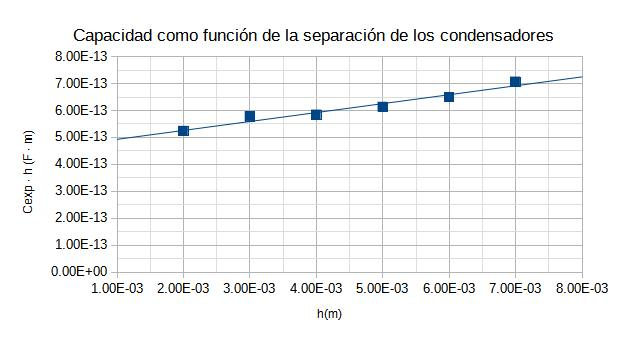
\includegraphics[width=\textwidth]{Grafica 1.jpg}

Con este procedimiento, se há encontrado con bastante precisión la capacidad parásita, $C_p$, que será utilizada en los cálculos posteriores de $\epsilon_0$. Para este último, se há obtenido una aproximación inicial que difiere del valor teórico en apenas un $2.15\%$. 

Ahora, se tiene como objetivo principal hacer el cálculo final de $\epsilon_0$ más preciso, y para esto es necesario considerar los efectos de borde. Como se había mencionado anteriormente, la idea básica es considerar más la geometría del condensador que en la ecuación ingénua, utilizando la llamada aproximación de Kirchoff para efectos de borde. De esta manera, se tiene que:

\begin{equation}
    C = \epsilon_0 F.G. = \epsilon_0 \left\{ \frac{\pi R^2}{h} \left[ 1+\frac{h}{\pi R} \left(\ln{\frac{16\pi R}{h}} -1 \right) \right] \right\}
\end{equation}

De donde se puede concluir que:

\begin{equation}
    C_{exp} - C_p = \epsilon_0 \cdot F.G.
\end{equation}

O sea, si se hace $C_{exp} - C_p$ como función de $F.G.$, la pendiente de esta regresión lineal será exactamente el coeficiente $\epsilon_0$. Repitiendo el procedimiento anterior para más valores de h, se tiene que:
\pagebreak

\begin{table}[h!]
    \centering
    \title{\textbf{Datos experimentales de la capacidad para diferentes separaciones para el cálculo de la permisividad del vacío.}}
    \begin{tabular}{|r|r|r|r|l|} 
    \hline
    \multicolumn{1}{|l|}{$h(m)$} & \multicolumn{1}{l|}{$C_{exp(F)}$} & \multicolumn{1}{l|}{$C_{exp}-C_p(F)$} & \multicolumn{1}{l|}{$F.G.(m)$} & \multirow{15}{*}{$\epsilon_0 = 8.85\cdot 10^{-12}$ F/m}  \\ 
    \cline{1-4}
    5.00$\cdot 10^{-3}$                   & 1.26$\cdot 10^{-10}$                     & 9.33$\cdot 10^{-11}$                        & 11.42             &                                         \\ 
    \cline{1-4}
    1.00$\cdot 10^{-2}$                   & 7.76$\cdot 10^{-11}$                     & 4.46$\cdot 10^{-11}$                        & 6.02             &                                         \\ 
    \cline{1-4}
    1.50$\cdot 10^{-2}$                   & 6.12$\cdot 10^{-11}$                     & 2.82$\cdot 10^{-11}$                        & 4.20             &                                         \\ 
    \cline{1-4}
    2.00$\cdot 10^{-2}$                   & 5.40$\cdot 10^{-11}$                     & 2.1$\cdot 10^{-11}$                         & 3.28             &                                         \\ 
    \cline{1-4}
    2.50$\cdot 10^{-2}$                   & 4.75$\cdot 10^{-11}$                     & 1.45$\cdot 10^{-11}$                        & 2.72             &                                         \\ 
    \cline{1-4}
    3.00$\cdot 10^{-2}$                   & 4.64$\cdot 10^{-11}$                     & 1.34$\cdot 10^{-11}$                        & 2.34             &                                         \\ 
    \cline{1-4}
    3.50$\cdot 10^{-2}$                   & 4.45$\cdot 10^{-11}$                     & 1.15$\cdot 10^{-11}$                        & 2.07             &                                         \\ 
    \cline{1-4}
    4.00$\cdot 10^{-2}$                   & 4.17$\cdot 10^{-11}$                     & 8.7$\cdot 10^{-12}$                         & 1.86              &                                         \\ 
    \cline{1-4}
    4.50$\cdot 10^{-2}$                   & 3.93$\cdot 10^{-11}$                     & 6.3$\cdot 10^{-12}$                         & 1.70             &                                         \\ 
    \cline{1-4}
    5.00$\cdot 10^{-2}$                   & 3.82$\cdot 10^{-11}$                     & 5.2$\cdot 10^{-12}$                         & 1.57             &                                         \\ 
    \cline{1-4}
    5.50$\cdot 10^{-2}$                   & 3.72$\cdot 10^{-11}$                     & 4.2$\cdot 10^{-12}$                         & 1.46              &                                         \\ 
    \cline{1-4}
    6.00$\cdot 10^{-2}$                   & 3.64$\cdot 10^{-11}$                     & 3.4$\cdot 10^{-12}$                         & 1.36             &                                         \\ 
    \cline{1-4}
    6.50$\cdot 10^{-2}$                   & 3.66$\cdot 10^{-11}$                     & 3.6$\cdot 10^{-12}$                         & 1.29             &                                         \\ 
    \cline{1-4}
    7.00$\cdot 10^{-2}$                   & 3.62$\cdot 10^{-11}$                     & 3.2$\cdot 10^{-12}$                         & 1.22            &                                         \\
    \hline
    \end{tabular}
\end{table}


\begin{tcolorbox}
    \begin{equation}
        \epsilon_0 = 8.85 \cdot 10^{-12} F/m
    \end{equation}
\end{tcolorbox}

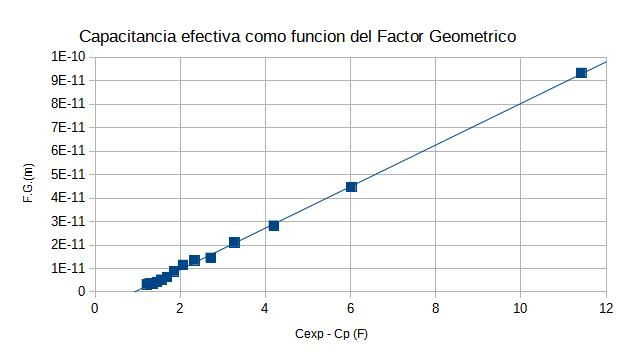
\includegraphics[width=\textwidth]{G2.jpg}

De esta manera, finalmente se ha obtenido un valor extremadamente preciso para $\epsilon_0$, idéntico al valor teórico presente en tablas de constantes comunes\footnote{Como un ejemplo, se tiene \cite[1420]{Tipler}} para el número de cifras significativas consideradas.

Finalmente, se pueden utilizar otros dieléctricos para obtener sus constantes y hacer otros cálculos de interés. Por ser apenas posible hacer una medida (con la separación igual a la grosura del dieléctrico), obviamente no serán las medidas más precisas, pero se puede tener una buena idea y ilustrar conceptos importantes:

\begin{center}
    \textbf{Datos experimentales de la capacidad para diferentes dieléctricos con el cálculo de los coeficientes relevantes}
\end{center}
\begin{table}[h!] 
    \centering
    \begin{tabular}{|l|r|r|r|r|r|r|} 
    \cline{2-7}
    \multicolumn{1}{l|}{}& \multicolumn{1}{l|}{$h(m)$} & \multicolumn{1}{l|}{$C_{exp}(F)$} & \multicolumn{1}{l|}{$C_{exp}-C_p(F)$} & \multicolumn{1}{l|}{$F.G.(m)$} & \multicolumn{1}{l|}{$\epsilon (F/m)$} & \multicolumn{1}{l|}{$\epsilon_r$}  \\ 
    \hline
    Vidrio            & 2.40$\cdot 10^{-3}$                  & 9.72$\cdot 10^{-10}$                     & 9.39$\cdot 10^{-10}$                        & 23.02             & 4.08$\cdot 10^{-11}$              & 4.60                 \\ 
    \hline
    Mármol          & 2.00$\cdot 10^{-2}$                  & 2.47$\cdot 10^{-10}$                     & 2.14$\cdot 10^{-10}$                       & 3.28             & 6.54$\cdot 10^{-11}$              & 7.39                 \\ 
    \hline
    Vidrio + Mármol  & 2.24$\cdot 10^{-2}$                  & 2.16$\cdot 10^{-10}$                     & 1.83$\cdot 10^{-10}$                       & 2.98             & 6.14$\cdot 10^{-11}$              & 6.94                 \\ 
    \hline
    ½ Vidrio + ½ Aire & 3.60$\cdot 10^{-3}$                  & 4.99$\cdot 10^{-10}$                     & 4.66$\cdot 10^{-10}$                       & 15.59             & 2.99$\cdot 10^{-11}$              & 3.37                 \\
    \hline
    \end{tabular}
\end{table}

Es importante mencionar que los condensadores del Vidrio+Mármol están en série y el de ½ Vidrio + ½ Aire en paralelo. De hecho, se puede ver que se verifica las relaciones esperadas. Sea $C_i=C_{exp\ i} - C_p$, se puede percibir que, considerada la imprecisión de las medidas, se verifican las relaciones que se deberían verificar:

$$C_{V+M} =\left(\frac{1}{C_V} +\frac{1}{C_M} \right)^{-1} =1.74 \cdot 10^{-10}F$$

Valor bastante próximo al obtenido experimentalmente, de $C_{V+M} = 1.83\cdot 10^{-10}F$, si se considera que se hizo apenas una medida. Lo mismo se verifica para el en paralelo de vidrio y aire:

$$C_{V\parallel A} = C_V + C_A = \frac{F.G.}{2} \left( \epsilon_0+\epsilon_V \right) = 3.87\cdot 10^{-10}F$$
 Aunque de hecho es bastante diferente del valor obtenido experimentalmente,$C_{V\parallel A} = 4.66\cdot 10^{-10}$ es próximo suficiente para la precisión utilizada para ilustrar la regla para el cálculo de capacidades equivalentes para condensadores en série.

\section{Conclusiones y Discusión}
Considerando la precisión deseada en cada apartado, todos los resultados estabán confortablemente dentro de lo deseado, a excepción tal véz la capacidad del ½ Vidrio + ½ Aire que está de veras diferente de lo que se esperaba que fuera. La fuente más importante y clara de error en esta experiencia es, claramente, la medición de h, que necesitaba de precisión milimétrica, y, en menor proporción, de problemas asociados al medidor LCR.

Además de eso, ya se há detallado como las medidas para las capacidades de objetos en série y paralelos no están en contradicción con la teoría electromagnética, ilustrando su poder predictivo. Obviamente, si se introducirá un conductor de capacidad $C_C$ en série con las planchas conectadas en série, tendríamos una nueva capacidad equivalente de $C_{eq} = \left(\frac{1}{C_{V+M}} +\frac{1}{C_C} \right)^{-1}$ y se podría verificarla una vez y otra más que la fórmula continúa con su poder descriptivo. 

\printbibliography
\end{document}
